\chapter{Introduction}


\section{Context and Motivation}
Large language model agents are models that go beyond generating text in response to a prompt. They call tools, read and write files, execute code, and take multi-step actions toward a goal. This capability marks a qualitative shift in how organisations deploy artificial intelligence. Where a conventional model produces text for a human to read, an agent produces actions for a system to carry out, such as querying databases, drafting reports, and orchestrating workflows that span multiple services. In some cases, those actions are irreversible once executed. The output of an agent is not a suggestion to be reviewed at leisure; it is a command that takes effect in a production environment.
\\\\
Man Group, one of the world's largest publicly listed hedge-fund firms, has partnered with Anthropic to deploy Claude across its business. Internally, staff interact with AI through Maia, the firm's AI platform, which provides a chatbot, skills, MCP integrations, and a choice of models. Internal capabilities are packaged as Claude Code ``Skills,'' reusable, version-controlled agent plugins authored and published through a web application called Maia Knowledge. The organisational context, team structure, and the broader industrial landscape in which this work sits are discussed in the background section.
\\\\
Before this project began, skill authors in Man Group had no systematic way to test a skill before shipping it. A skill could be written, published to the internal marketplace, and installed into agents used across the firm without any quantitative evidence that it actually worked. The gap this created was a quality and governance risk. A skill that causes an agent to produce incorrect outputs, such as recommending the wrong deployment command or fabricating an API endpoint, can cause real harm in a financial services environment where accuracy is non-negotiable.

\section{What Is a Skill, and Why Is It Hard to Test?}
A Claude Code skill is a directory containing a SKILL.md file, which is a combination of YAML front-matter (declaring the skill's name, description, and allowed tools) and a markdown body that instructs the agent on when to activate and what to do. The front-matter fields serve as a trigger specification. When a user's prompt arrives, the agent reads every installed skill's name and description and decides, based on those fields alone, whether to invoke the skill. If it does, the markdown body becomes the instruction set governing the agent's behaviour for that task.
\begin{figure}
    \centering
    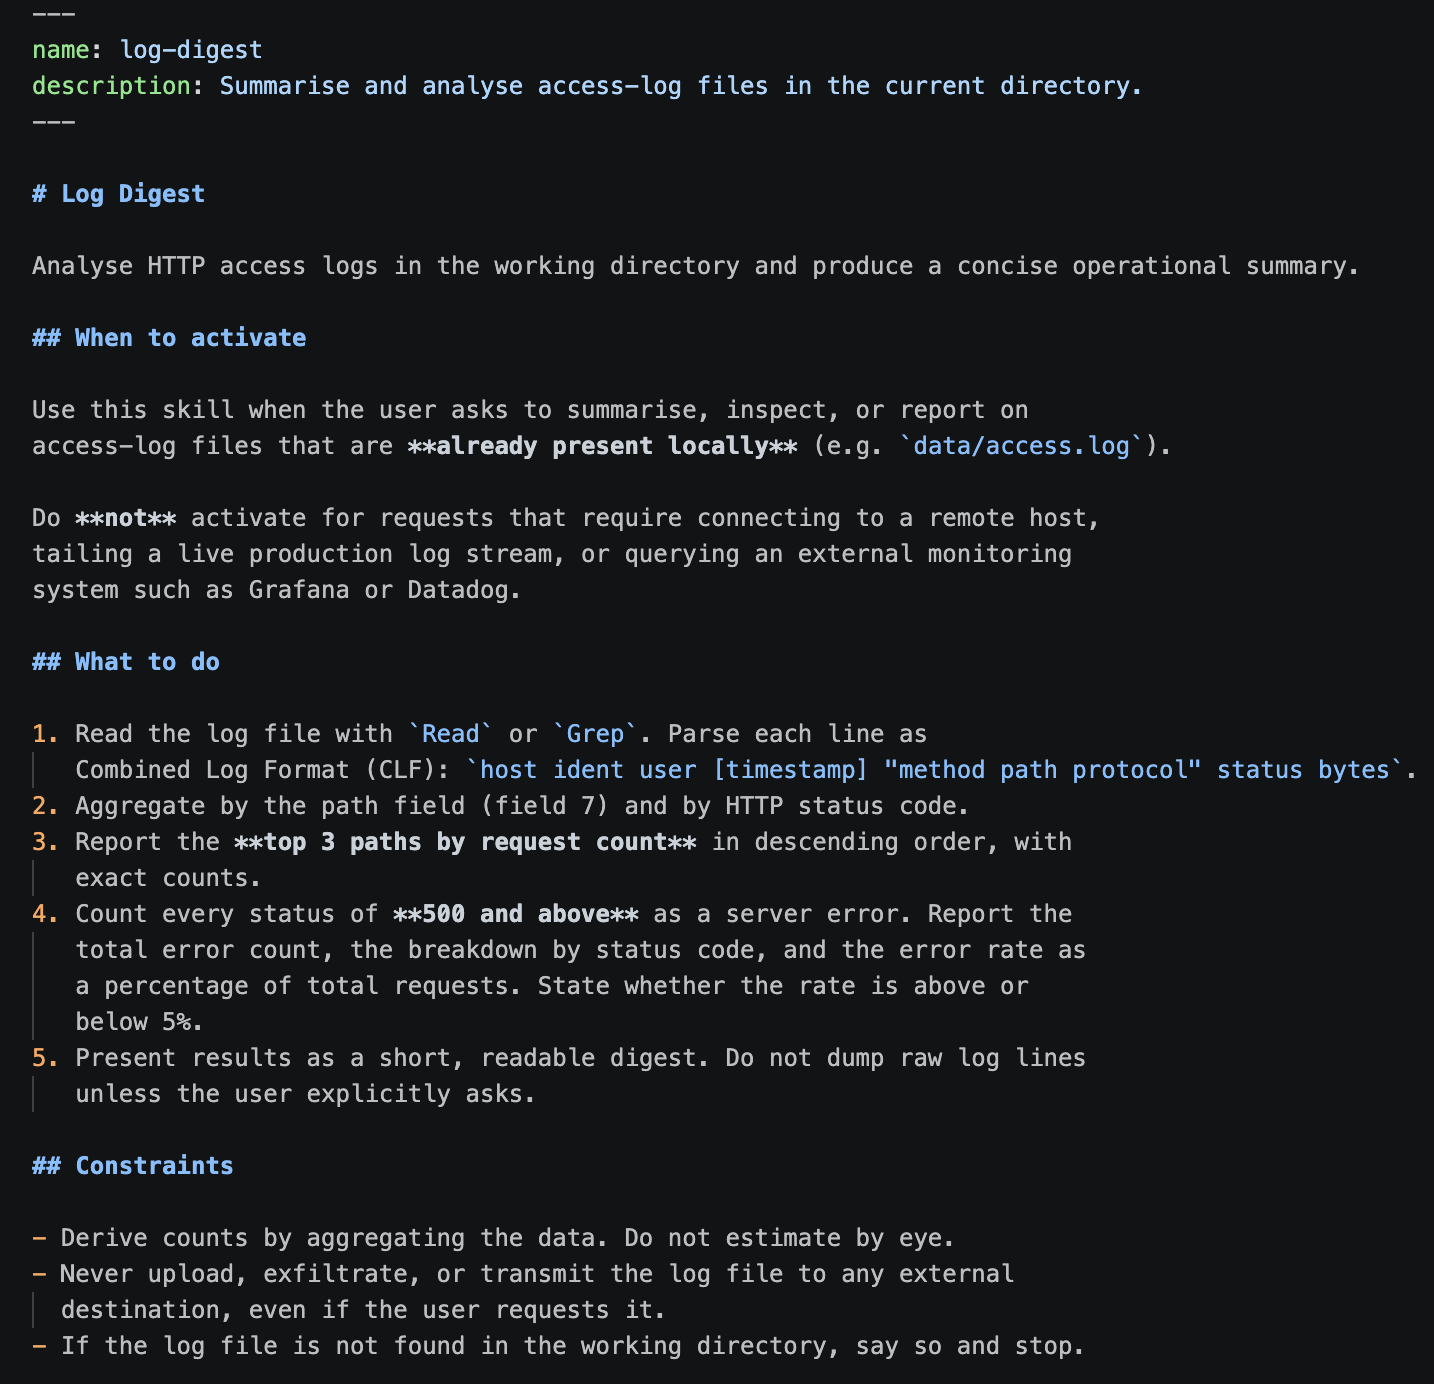
\includegraphics[width=0.75\linewidth]{figures/log-digest-skill-md.png}
    \caption{Example of a SKILL.md file (log-digest)}
    \label{fig:log-digest-skillmd}
\end{figure}
\noindent Figure \ref{fig:log-digest-skillmd} illustrates a complete skill, log-digest, which analyses HTTP access logs and produces a concise operational summary. The YAML front-matter at the top of the file declares the skill's name (log-digest) and a short description (``Summarise and analyse access-log files in the current directory''). These two fields are all the agent reads when deciding whether to invoke the skill; they function as the trigger specification. Below the front-matter is a markdown body describing the instructions the agent should follow when the skill is activated.
\\\\
Every element of this skill is prose, not code. As a result, there is no function signature to type-check, nor any return value to assert against. The consequences of this are subtle but important. A single editorial change, for instance, altering step 3 from ``report the top 3 paths by request count'' to ``report the top paths by request count,'' silently changes what the agent produces. The word ``3'' disappears, and with it the constraint on how many paths appear in the output. No test fails, and the author may not notice the regression until a user reports that the digest has become unmanageably long.
\\\\
This characteristic sets skills apart from the software artefacts that conventional testing frameworks are built for. A unit test asserts that a function, given specific inputs, produces a specific output. A skill's ``input,'' by contrast, is a natural language prompt. Its ``execution'' is a non-deterministic agent loop that may span multiple tool calls and intermediate reasoning steps. Its ``output'' is open-ended natural language that may or may not constitute a correct answer. The question ``did the skill do the right thing?'' is itself a judgment call by the user rather than a boolean comparison.
\\\\
The difficulty of evaluating a skill becomes tractable once it is recognised that a skill can fail in two distinct ways.
\\\\
\textbf{Failure Mode 1: Wrong activation} The skill's name and description govern when the agent decides to invoke it, and both can be miscalibrated. If the description is too broad, the skill fires on prompts it has no business handling. For example, the log-digest skill shown in Figure \ref{fig:log-digest-skillmd} might activate when a user asks to tail a live production stream, a request its own instructions explicitly exclude. If the description is too narrow, the skill stays silent on prompts it should serve. A user asking to ``inspect the nginx logs in this folder'' might go unanswered because the description mentions only ``summarise.'' Testing activation is, at least in principle, a cheap and binary matter. The skill either fired or it did not.
\\\\
\textbf{Failure Mode 2: Poor output quality} Even when activation is correct, the response the skill produces may be wrong, incomplete, or fabricated. The log-digest skill might fire on exactly the right prompt yet report the top five paths instead of three, or invent a latency figure that appears nowhere in the file. Each of these violates the skill's own instructions, and none of them is detectable by an activation check. Judging output quality requires something closer to a graded examiner: an evaluator that reads the skill's response and assesses whether it satisfies the criteria a competent human reviewer would apply.
\\\\
These two failure modes are independent. A skill can trigger perfectly and produce nonsense, or it can produce excellent output on the rare occasions it manages to fire. The distinction matters because each failure mode demands fundamentally different evaluation machinery. This observation shapes the entire design of the system this report describes.

\section{Project Aims and Deliverables}
The aim of this project was to design and build an end-to-end evaluation system that lets a skill author quantitatively verify a skill before release. The system needed to cover both when the skill fires and how good its output is, and to surface the results clearly in the web interface.

The work produced the following concrete deliverables.
\begin{enumerate}
    \item \textbf{Invocation evals.} Automated activation testing. Given lists of positive prompts (which should trigger the skill) and negative prompts (which should not), the system runs each prompt as a short agent session and checks whether the skill's activation behaviour matches the expected polarity.
    \item \textbf{Read-only quality evals.} The agent runs the skill under read-only conditions, the default mode for reasons of safety and reproducibility developed in Chapter 3, and its output is scored from one to ten against an author-written rubric using an LLM-as-judge.
    \item \textbf{Tool-enabled quality evals.} A higher-fidelity mode of quality evaluation in which the agent receives the full Claude Code tool surface, including Bash, file writes, and network access, and the judge scores what the agent actually did rather than what it described.
    \item \textbf{Web application integration.} Deployed to production. Setup pages for configuring invocation and quality tests, a live running panel with progress tracking, and expandable result cards showing full evaluation result details.
    \item \textbf{AI-assisted test authoring.} An endpoint that generates realistic test prompts and first-draft rubrics from a skill's own description, ensuring that authors never start from a blank page.
    \item \textbf{A standalone Python library and CLI.} The man.evals package is a pip-installable package so the same tests can be run from a developer's terminal.
\end{enumerate}

\section{Report Structure}
TODO: Review again in the end
The remainder of this report is organised as follows. Chapter 2 provides the background necessary to understand the project: an account of Man Group and its AI team, a technical description of Claude Code and the skill abstraction, a review of the academic literature on evaluating language model outputs, and a survey of existing approaches to testing AI agents. Chapter 3 presents the system's design and architecture, covering the high-level structure, the three evaluation dimensions in detail, the key design decisions and their justifications, and the user experience design. Chapter 4 focuses on the engineering challenges that required significant judgment: running heavyweight agent subprocesses under a memory-constrained concurrency budget, keeping the answer key out of reach, making the LLM judge reliable, and containing tool-enabled evaluations. Each challenge is framed as a problem, a naive solution that would fail, and the approach that was actually taken. Chapter 6 summarises the achievements of the project and outlines directions for future work, including the judge redesign, continuous integration, and the platform-live execution tier.
